\documentclass[11pt]{article}
\usepackage[english]{babel}
\usepackage[utf8]{inputenc}
\usepackage{fancyhdr}
\usepackage{graphicx}

\def\Name{Ran Liao}
\def\Topic{Computer Networks}

\title{\textbf{\Topic}}
\author{\Name}
\markboth{Notes on \Topic\ }{Notes on \Topic\ }
\date{\today}
 
\pagestyle{fancy}
\fancyhf{}
\rhead{\date{\today} }
\lhead{Notes on \Topic\ }
\rfoot{\thepage}

\textheight=9in
%\textwidth=6.5in
\topmargin=-.75in
%\oddsidemargin=0in
%\evensidemargin=0in
 
\begin{document}
\maketitle
\tableofcontents
\newpage

\section{Introduction}

In Internet jargon, all of these devices are called \textbf{hosts} or end \textbf{systems}.
End systems are connected together by a network of \textbf{communication links} and \textbf{packet switches}.
Packet switches come in many shapes and flavors, but the two most prominent types in today’s Internet are \textbf{routers} and \textbf{link-layer switches}.
The sequence of communication links and packet switches traversed by a packet from the sending end system to the receiving end system is known as a \textbf{route} or \textbf{path} through the network.
End systems access the Internet through \textbf{Internet Service Providers (ISPs)}.

\section{Circuit Switching versus Packet Switching}

There are two fundamental approaches to moving data through a network of links and switches: \textbf{circuit switching} and \textbf{packet switching}. 

\subsection{Packet Switching}

In a network application, end systems exchange messages with each other. To send a message from a source end system to a destination end system, the source breaks long messages into smaller chunks of data known as \textbf{packets}. Between source and destination, each packet travels through communication links and packet switches.

\subsection{Circuit Switching}

In circuit-switched networks, the resources needed along a path (buffers, link transmission rate) to provide for communication between the end systems are \textit{reserved} for the duration of the communication session between the end systems.


\subsubsection{FDM : Frequency-Division Multiplexing}
	
	With FDM, the frequency spectrum of a link is divided up among the connections established across the link. Specifically, the link dedicates a frequency band to each connection for the duration of the connection.
	
\subsubsection{TDM : Time-Division Multiplexing}
	
	For a TDM link, time is divided into frames of fixed duration, and each frame is divided into a fixed number of time slots. When the network establishes a connection across a link, the network dedicates one time slot in every frame to this connection. These slots are dedicated for the sole use of that connection, with one time slot available for use (in every frame) to transmit the connection’s data.
	
\begin{figure}[h]
	\centering
	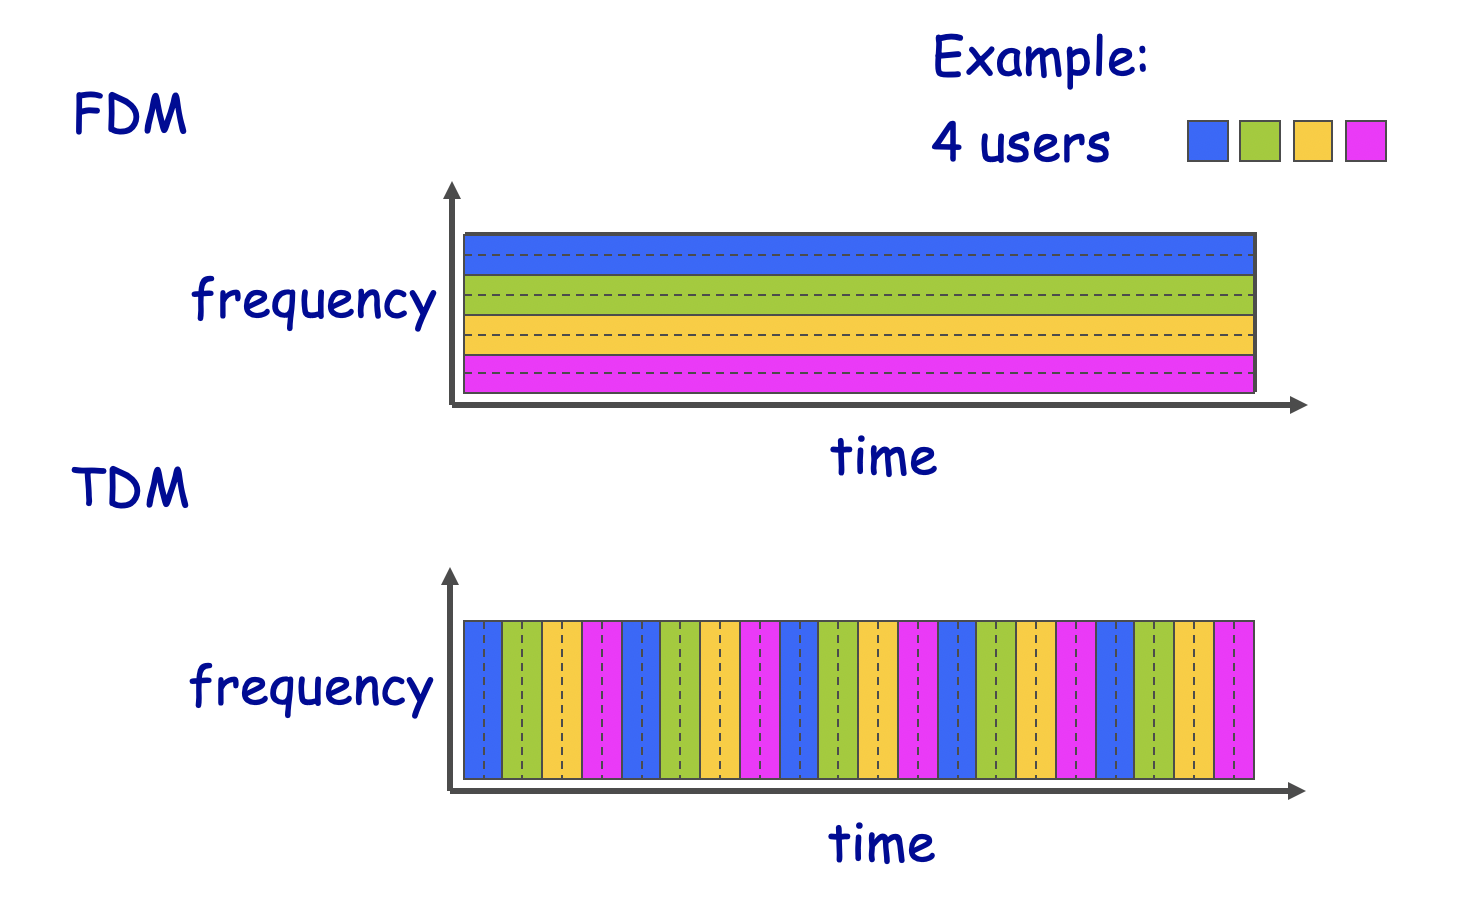
\includegraphics[width=0.8\linewidth]{images/FDMvsTDM.png}
	\caption{FDM versus TDM}
	\label{fig:FDMvsTDM}
\end{figure}

\subsection{Trade-off}

Packet Switching is not suitable for real-time services because of its variable and unpredictable end-to-end delays (due primarily to variable and unpredictable queuing delays). Proponents of packet switching argue that (1) it offers better sharing of transmission capacity than circuit switching and (2) it is simpler, more efficient, and less costly to implement than circuit switching.

Circuit switching pre-allocates use of the transmission link \textit{regardless of demand}, with allocated but unneeded link time going unused. Packet switching on the other hand allocates link use \textit{on demand}. Link transmission capacity will be shared on a packet-by-packet basis only among those users who have packets that need to be transmitted over the link.

\section{Delay}

Denote $d_{proc}$, $d_{queue}$, $d_{trans}$, and $d_{prop}$ to be the processing, queuing, transmission, and propagation delays respectively. Then the total nodal delay is given by

\[
	d_{nodal} = d_{proc} + d_{queue} + d_{trans} + d_{prop}
\]

\subsection{Processing Delay}

The time required to examine the packet’s header and determine where to direct the packet is part of the processing delay.

\subsection{Queuing Delay}

Each packet switch has multiple links attached to it. For each attached link, the packet switch has an \textbf{output buffer} (also called an \textbf{output queue}), which stores packets that the router is about to send into that link. If an arriving packet needs to be transmitted onto a link but finds the link busy with the transmission of another packet, the arriving packet must wait in the output buffer. The \textbf{queuing delays} is the time packet waits to be transmitted in the output queue. These delays are variable and depend on the level of congestion in the network. 

Since the amount of buffer space is finite, an arriving packet may find that the buffer is completely full with other packets waiting for transmission. In this case, \textbf{packet loss} will occur --- either the arriving packet or one of the already-queued packets will be dropped.

Denote $a$ to be the average rate at which packets arrive at the queue (in units of packets/sec). The ratio $\frac{aL}{R}$ is called the \textbf{traffic intensity}. If  $\frac{aL}{R} > 1$, then the average rate at which bits arrive at the queue exceeds the rate at which the bits can be transmitted from the queue. In this unfortunate situation, the queue will tend to increase without bound and the queuing delay will approach infinity.

\subsection{Transmission Delay}

Most packet switches use \textbf{store-and-forward transmission} at the inputs to the links. Store-and-forward transmission means that the packet switch must receive the entire packet before it can begin to transmit the first bit of the packet onto the outbound link. Consider the general case of sending one packet of $L$ \textit{bits} over a link with rate $R$ \textit{bits/sec}. Then the \textbf{transmission delay} is $\frac{L} {R}$ \textit{seconds}.

\subsection{Propagation Delay}

The propagation delay is the distance between two routers divided by the propagation speed. The propagation speed depends on the physical medium of the link and is in the range of $2 \cdot 10^8$ \textit{meters/sec} to $3 \cdot 10^8$ \textit{meters/sec}.

\subsection{Clarification}

The \textbf{transmission delay} is the amount of time required for the router to push out the packet; it is a function of the packet’s length and the transmission rate of the link, but has nothing to do with the distance between the two routers. The \textbf{propagation delay}, on the other hand, is the time it takes a bit to propagate from one router to the next; it is a function of the distance between the two routers, but has nothing to do with the packet’s length or the transmission rate of the link.

\section{Protocol Layers and Their Service Models}

To provide structure to the design of network protocols, network designers organize protocols—and the network hardware and software that implement the protocols— in \textbf{layers}. We are interested in the \textbf{services} that a layer offers to the layer above—the so-called \textbf{service model} of a layer. When taken together, the protocols of the various layers are called the \textbf{protocol stack}.

\subsection{Application Layer}

The application layer is where network applications and their application-layer protocols reside. The Internet's application layer includes many protocols, such as the HTTP, SMTP, FTP and DNS.

\subsection{Transport Layer}

The Internet’s transport layer transports application-layer messages between application endpoints. In the Internet there are two transport protocols, TCP and UDP, either of which can transport application-layer messages. TCP provides a connection-oriented service to its applications, whereas the UDP protocol provides a connectionless service to its applications. 

\subsection{Network Layer}

The Internet’s network layer is responsible for moving network-layer packets known as datagrams from one host to another.

\subsection{Link Layer}

The Internet’s network layer routes a datagram through a series of routers between the source and destination. To move a packet from one node (host or router) to the next node in the route, the network layer relies on the services of the link layer.

\subsection{Physical Layer}

While the job of the link layer is to move entire frames from one network element to an adjacent network element, the job of the physical layer is to move the individual bits within the frame from one node to the next.

\section{Security Threat}

\begin{itemize}
	\item \textbf{Denial-of-Service (DoS)}
	\item \textbf{Sniffing}
	\item \textbf{Spoofing}
\end{itemize}

\end{document}